% !TeX root = ../main.tex

\chapter{Approach}\label{chapter:approach}
The purpose of the tool is the continuous detection of copied code in a changing codebase.
The work of Koschke et al. makes clear that a index based approach seems appropriate for continuous detection:
\glqq If the [copy-paste detection] analysis is to be conducted multiple times, creating an index pays off\grqq \cite{koschke2014large}.

This chapter describes the followed approach and architecture of the tool in detail.

\section{System Overview}
\begin{figure}[h]
	\centering
	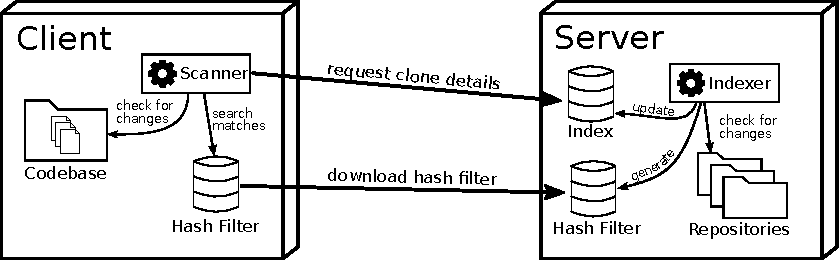
\includegraphics{figures/architecture_overview.pdf}
	\caption{Tool Architecture Overview}\label{fig:tool_architecture}
\end{figure}
\autoref{fig:tool_architecture} shows an overview of the tool's client-server architecture.
The servers purpose is to provide a lookup service for code.
The client has code which should be checked for license infringements and can use this service to find similar code in open source systems.
The server has access to a pool of repositories and creates the index by normalizing and hashing files of the repositories as described in section \ref{section:approach/creating_index/normalization}.
Subsequently, the history of a reference system is analyzed as explained in section \ref{section:approach/creating_index/history_analysis}.
After that, the server generates the filter as described in section \ref{section:approach/creating_index/hash_filter}.

The client's search is two staged as described in \autoref{section:approach/searching_copied_code}
First the Scanner on the client normalizes and hashes files in its codebase the same way the server does.
In the first stage, the hash filter is used to exclude hashes, which are not part of the server's index.
The hash filter can be downloaded from the server.
The second stage then requests the clone details from the server for the remaining hashes.
This can be done in a continuous manner, i.e. with every change on the client's codebase.

\section{Creating the Index}\label{section:approach/creating_index}
The index is based on the work of Hummel et al. \cite{hummel2010index}, where normalized sequences of statements of the code, which are called chunks, are hashed.
Other chunks of code can then be looked up by calculating the hash of those chunks the same way.
By comparing the resulting hashes with hashes in the index, locations of similar code can be found.

This section describes the process which is done to create the index.

To add a source code file to the index, it first is parsed and split into tokens.
A token represents a small part of the code such as a symbol, keyword, identifier, literal or comment.
The tokens then are normalized as described in \autoref{section:approach/creating_index/normalization}.
Now the tokens are aggregated into statements.
The tool then passes over the resulting list of statements using a sliding window to group together a chunk of code, which consists of several consecutive statements.
The amount of statements in a chunk influences the precision of a match, since longer chunks also require longer matches.

The resulting chunks could be used to find similar code segments.
To reduce the space needed to store the information needed to identify similar code, the chunks are hashed.
\autoref{fig:normalization} shows the complete processing of an input file.

Hashes and their originating chunk are stored in a database.

\subsection{Normalization}\label{section:approach/creating_index/normalization}
The normalization step removes irrelevant information and by that, concentrates on the essential features of the code.
The parsing of code into tokens already does the first part of normalization by removing formatting.
After that, irrelevant tokens like access modifiers, import or include statements, comments or symbols like brackets or semicolons are removed.
The tokens which are left contain the main portion of information relevant for comparison of two sequences of code.
Since the tool should uncover mainly directly copied code, no further normalization is done.

\subsection{History Analysis}\label{section:approach/creating_index/history_analysis}
It is important to also index old versions of the reference system.
Otherwise code, which has been copied from older versions of an open source system may not be detected.

To keep the index up to date and still keep information about older versions of the file, changed files of reference systems are re-indexed.
For that, the server normalizes the new version of the file the same way as described before, groups it into chunks and hashes those chunks.
The resulting hashes are then inserted into the key value store.
If a hash already exists and links to a file with the same location, the old link is replaced with the new one to save space.
This ensures, that a hash always points to the latest version of a file.
When files are deleted, nothing is changed in the key value store.

Instead of rescanning the whole file, only the chunks which have changed could be scanned.
However, the locations of hashes for chunks which did not change also have to be updated  in order to keep the latest version of a file in the index.


\subsection{Hash Filter}\label{section:approach/creating_index/hash_filter}
It is expected, that most of the calculated hashes of a target system can not be found in the index.
Instead of having to send a request for every hash to the server, a better option would be a local copy of the index for faster lookup.
However, since the index may contain hashes and the according location for billions lines of code, it is huge.
Distribution of the index to clients is a challenge, especially since the index has to be updated regularly.

With a table of all hashes, which are contained in the index, the client would be able to lookup whether a hash is in the index and only has to send a request to the server in this rare case.
This could significantly speed up the analysis, since only hashes which actually are in the index would be looked up.
On the server-side this also reduces the load.

The size of the hash table is the amount of hashes times 128 bits which is the length of a MD5 hash.
Hashing with MD5 reduces the entropy of a chunk to about 128 bit of a ideal hash function.
Since lossless compression is expected not to reduce the size of the hashtable by much, lossy compression could be used.
One great way of reducing size of hash table with low false-positive probability is a BloomFilter.

To store a value, a BloomFilter uses multiple hash functions to hash a value\cite{bloom1970filter}.
It uses the resulting hash values as indexes to set bits of a bit array to 1.
To find out whether a value is stored in the BloomFilter, the value is hashed with the same hash functions as for storing a value.
Again, hash values are used as indexes.
If all values inside the bit array defined by the indexes are set to 1, the value is stored in the BloomFilter with a high probability.
If one or more of the bits are not set, the value is guaranteed not in the filter.
For the tool developed in this work, the values inserted into the BloomFilter are the hashes of the chunks.

%TODO: "By making a sparse Bloom filter using 48 bits per element but only 3 hash functions, one can compress the result down to less than 16 bits per item with high probability) and decrease the false positive probability by roughly a factor of 2. @Mitzenmacher, Michael; Upfal, Eli (2005), Probability and computing: Randomized algorithms and probabilistic analysis S.10

The advantage here is the small size of the filter.
However, the compression is lossy, because there is a certain probability for false positives.
The probability is depending on the size of the bit array, the number of inserted values and the number of used hash functions, but when kept at an optimum, grows almost (due to discrete number of hashing functions) linearly with the number of insertions.
Since it is not possible to remove values from the filter, it has to be recalculated every time the index changes.

It is also possible to only use the filter to find potential copied code.
This however, does not allow the client to find the origin for a potential match.
	
\section{Searching Copied Code}\label{section:approach/searching_copied_code}
The client has a codebase which should be searched for copied code.
To do so, it normalizes the code in question, groups statements and hashes them as described in \autoref{section:approach/creating_index}.
\begin{itemize}
	\item TODO Activity diagram: client <-> server
	\item TODO calculate probability of final false positive
\end{itemize}

\section{Future Work / Extensibility}\label{section:approach/extensibility}
\begin{itemize}
	\item TODO Use Cuckoo-Filter \cite{fan2014cuckoo} instead of Bloom-Filter. Better performance in low false-positive probability with many items
	\item TODO Optimize normalization: Method based?, block-based => switch methods/structs/enums positions
	\item TODO Assess matches: Load file(s) from server, do more comparison (With a difftool token based on methods/blocks, to prevent reordering of methods not detected)
	\item TODO Extension points for future development? Web-Interface for code-add-request, Suggestions for linking libraries (gradle, ...)
\end{itemize}